\chapter{Theory and Related Work}
\label{chap:back}

In this second chapter, we establish the theoretical foundation for our work, covering key concepts in \acrshort{das} signal processing, anomaly detection, and \acrshort{ai}. Furthermore, we explore relevant data processing techniques and examine previous research on \acrshort{das} processing, anomaly detection and autoencoders, with a particular focus on methods applicable to \acrshort{das} data.

\section{Digital Signal Processing}

The field of \acrfull{dsp} has been researched since the dawn of time. Signals are all around us, and we do have the means to gather and store the data, but how do we process it more efficiently to be able to analyze and interpret the data in a fast and efficient manner.

When working with \acrshort{das} data in particular, we want to filter the data to remove distortion, and get cleaner outputs to work with. A common way to remove signals outside of a range are called High-pass filters and Low-pass filters. 

A high-pass filter is a function that only allows frequencies above a certain threshold to be accepted, while a low-pass filter only accepts frequencies lower than a threshold $T$. A band-pass filter on the other hand, only allows frequencies within a certain range to be accepted.

\begin{figure}[h]
\centering
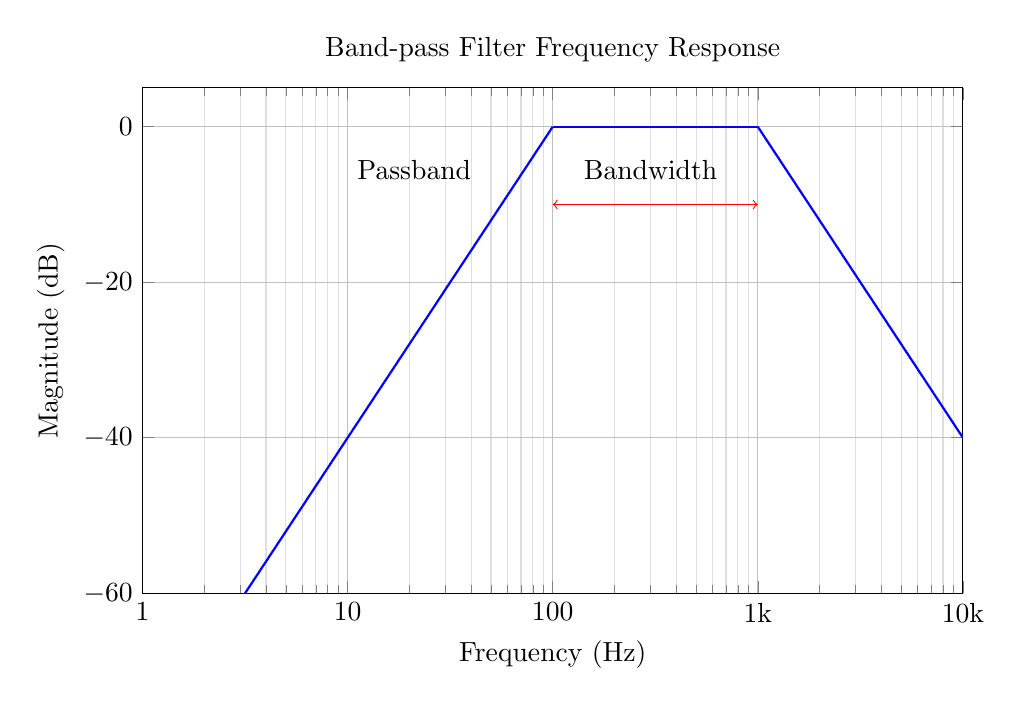
\begin{tikzpicture}
\begin{axis}[
    width=12cm,
    height=8cm,
    xlabel={Frequency (Hz)},
    ylabel={Magnitude (dB)},
    xmode=log,
    xmin=1, xmax=10000,
    ymin=-60, ymax=5,
    xtick={1,10,100,1000,10000},
    xticklabels={1,10,100,1k,10k},
    ytick={-60,-40,-20,0},
    grid=both,
    minor grid style={gray!25},
    major grid style={gray!50},
    title={Band-pass Filter Frequency Response},
]

% Low-frequency rolloff
\addplot[domain=1:100,samples=100,blue,thick] {-40*log10(100/x)};

% Passband
\addplot[domain=100:1000,samples=100,blue,thick] {0};

% High-frequency rolloff
\addplot[domain=1000:10000,samples=100,blue,thick] {-40*log10(x/1000)};

% Annotations
\node[anchor=north west] at (axis cs:10,-3) {Passband};
\draw[<->,red] (axis cs:100,-10) -- (axis cs:1000,-10);
\node[anchor=south] at (axis cs:300,-8) {Bandwidth};

\end{axis}
\end{tikzpicture}
\caption{Ideal Bandpass Filter Response}
\end{figure}


\subsection{Tukey Window}
\label{dsp:tukey}

Window functions are function often used in \acrshort{dsp} and are zero-valued outside of an interval. The Tukey window, also known as the \textit{cosine-tapered window} is one of the more popular window methods, and its mathematical function is described as such: 

\[
    w(x)= 
\begin{cases}
    \frac{1 + \cos{2 \pi \alpha (x + \frac{1-\alpha}{2})}}{2}, & \text{if } x \leq \frac{1-\alpha}{2}\\
    1,              & \text{if } \frac{\alpha}{2} < x \leq \frac{\alpha}{2}\\
    \frac{1 + \cos{2 \pi \alpha (x - \frac{1-\alpha}{2})}}{2}, & \text{if } x > \frac{1-\alpha}{2}
\end{cases}
\]

This window becomes a rectangle when $\alpha = 0$.


\subsection{Resampling}

Also known as sampling-frequency conversion, resampling is the act of modifying the sampling rate of a discrete signal to obtain a new discrete representation of this data. For signal data, lots of samples are usually recorded, but the amount needed to perform calculations or observe patterns does not require this much data. Thus, one can downsample the data to decrease memory usage for storage, as well as time for processing this data. \\


\subsection{Butterworth}

TBI.
\section{Deep Learning}

% Deep Learning
\acrfull{dl} is a subset of \acrshort{ml} and \acrshort{ai}, where the objective is to learn underlying representations of data \cite{lecun2015deep}. In \acrshort{dnn}s, neurons act as the fundamental building blocks. Layers of neurons are grouped into three categories of layers: input-, output- and \textit{hidden layers}.  

\begin{figure}[!h]
    \centering
    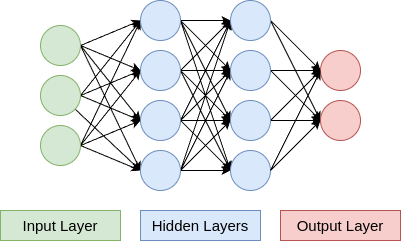
\includegraphics[width=0.5\linewidth]{figures/dnn.png}
    \caption{Example of a dense neural network with one input layer, two hidden layers and one output layer}
    \label{fig:densenn}
\end{figure}

We mainly differentiate between three subcategories of \acrshort{dl}:

\begin{itemize}
    \item \textit{Supervised learning}: Data is labeled, and the goal of the network is trained to make sure the outputs match these labels.
    \item \textit{Unsupervised learning}: The network learns patterns exclusively from unlabeled data and tries to learn the underlying structure of the input vectors \cite{KARHUNEN2015125}. 
    \item \textit{Semi-supervised learning}: Some data may be labeled
\end{itemize}



\subsection{Fully Connected Neural Networks}
\label{back:linear}

\acrfull{fcnn} are fundamental networks used in many \acrshort{dl} models. Also called dense or linear networks, they are characterized by all neurons being connected between two layers (see Figure \ref{fig:densenn}). 

In the forward pass, linear layers transform the input data, mapping an input vector to an output vector using learnable parameters. The operation can be defined as follows:
\begin{equation}\label{f:wxb}
    \mathbf{y} = \mathbf{w}x+b
\end{equation}
Here, $x$ is the input vector, \textbf{$w$} is the weight matrix, $b$ is the bias, and \textbf{$y$} is the output vector.

\begin{figure}[!h]
    \centering
    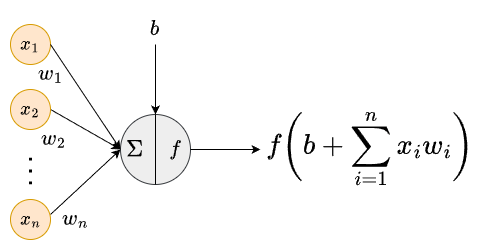
\includegraphics[width=0.7\linewidth]{figures/dl.png}
    \caption{Neurons $x$ in a layer with their weights $w$, a bias $b$ and an activation function $f$}
    \label{fig:dl}
\end{figure}

Furthermore, an activation function $f$ is applied to the output to achieve \textit{nonlinearity}. By applying $f$ to the output $y$, we now get the equation:
\begin{equation}\label{f:fwxb}
    \mathbf{z} = f(\mathbf{y}) = f(\mathbf{w}x+b)
\end{equation}

Some of the more popular activation functions include \cite{szandala2021review}: 

\begin{equation}
    Relu(z) = max(0, z)
\end{equation}

Relu (Rectified Linear Unit) was stated to be the most popular activation function as late as 2018. Its forward and backward pass steps quickly, thus enabling more efficient training compared to other alternatives.

\begin{equation}
    \sigma(z) = \frac{1} {1 + e^{-z}}
\end{equation}

The sigmoid activation is very popular because its range is $[0,1]$, compared to other functions, is rather limited and represents a probabilistic value. This makes it good at outputting probabilistic values.

\begin{equation}
    tanh(x) = \frac{e^x - e^{-x}}{e^x + e^{-x}} = \frac{1 - e^{-2x}}{1 + e^{-2x}}
\end{equation}

Like sigmoid, the hyperbolic tangent has outputs in a relatively small range $[-1, 1]$.

After the forward pass is performed, the network will update its weights. This is done by using a \textit{cost}, or \textit{loss} function and using the resulting loss to calculate the networks' gradients before an optimizer, such as \acrfull{sgd} \cite{Rumelhart1986, Bottou2012}, updates the weights before the following forward pass. For unsupervised networks specifically, two of the more commonly used loss functions include: \\

\textbf{\acrfull{mse}}

\begin{equation}\label{eq:mse}
    \mathcal{L}_{\text{MSE}}(x, \hat{x}) = \dfrac{1}{N}  \sum_{i=1}^{N}(x_i-\hat{x}_i)^2
\end{equation}

The \acrshort{mse} loss function is a commonly used loss function. It punishes bigger differences by squaring the difference between two elements in the prior $x$ and the posterior $\hat{x}$. It then outputs the mean of all the squarred errors computed. \\

\textbf{\acrfull{mae}}

\begin{equation}\label{eq:mae}
    \mathcal{L}_{\text{MAE}}(x, \hat{x}) = \dfrac{1}{N}  \sum_{i=1}^{N}|x_i-\hat{x}_i|
\end{equation}

The \acrshort{mae} loss function is similar to the \acrshort{mse} function. The difference is that the \acrshort{mae} function returns the absolute value of the distance between two distributions $x$ and $\hat{x}$, thus equally punishing all errors. \\

The major bottleneck of all kinds of machine learning techniques is data. The more diverse and varied a . \\

Linear layers have several advantages, such as computational efficiency, flexibility as well as intrerprebility, where the weight and bias vectors can be interpreted as learned parameters. They also serve as building blocks for other components, such as \acrshort{rnn}s \cite{schmidt2019recurrent}, \acrshort{lstm}s \cite{lstm} or even more novel architectures such as the transformer\cite{vaswani2017attention}. \\ 

However, linear layers have several limitations. Due to their inherent linearity, they are prone to \textit{overfitting} and struggle to capture complex relationships in data. This can limit their ability to extract more complex features, potentially reducing some of the model's discriminative power. Furthermore, the size of linear layers can become problematic, especially in \acrshort{fcnn}s. Each neuron connection between layers requires storing weights and biases, which increases the overall model size. For a smaller dense network where the layers are of size $[10, 5, 1]$, the total amount of parameters becomes:
$$\begin{aligned}
S &= (10 \times 5 + 5) + (5 \times 1 + 1) \
&= 50 + 5 + 5 + 1 \
&= 61 \text{ parameters}
\end{aligned}$$
Assuming each parameter is stored as a single-precision floating-point number (\texttt{Float32}, 4 bytes), the total memory size is:
$$\begin{aligned}
\text{Memory size} &= 61 \text{ parameters} \times 4 \text{ bytes/parameter} \
&= 244 \text{ bytes}
\end{aligned}$$ While 244 bytes is small, larger dense networks can quickly consume gigabytes of memory. This can create bottlenecks for hardware accelerators like \acrshort{gpu}s, which typically have less VRAM compared to the \acrshort{ram} available to \acrshort{cpu}s.
\subsection{CNN - Convolutional Neural Networks}
\label{back:cnn}

\acrfull{cnn} \cite{}, a specialized type of feed-forward neural network, has become a cornerstone in \acrshort{dl} architectures. Building upon simpler structures like the linear layer discussed in section \ref{back:linear}, CNNs introduce a powerful approach to processing matrix data, especially images.
The foundations of CNNs can be traced back to neurobiological research in the 1960s on the visual cortex \cite{hubel1962receptive}, but they were first properly introduced to the \acrshort{ml} field in 1990 by Yan LeCun \cite{NIPS1989_53c3bce6}. Since then, CNNs have undergone significant developments, leading to breakthroughs in various fields of artificial intelligence. \\

\begin{figure}[!h]
    \centering
    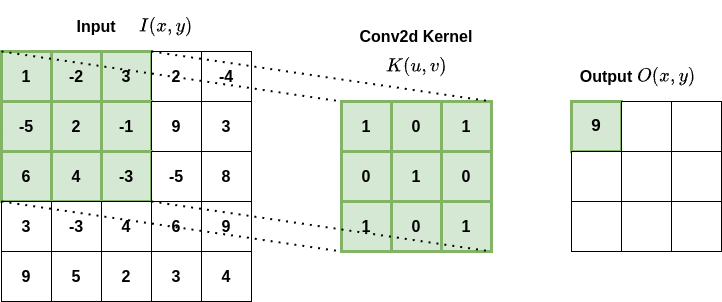
\includegraphics[width=0.8\linewidth]{figures/convolution.png}
    \caption{Example of a 2D Convolutional operation}
    \label{fig:2dconv}
\end{figure}

At their core, CNNs rely on kernel operations, primarily convolutions, to calculate features. The convolution is a mathematically operation which can be defined continuously as following:

\begin{equation}
(f * g)(t) = \int_{-\infty}^{\infty} f(\tau) g(t - \tau) d\tau
\label{eq:contconv}
\end{equation}

and discretely as such:

\begin{equation}
   (f * g)(x, y) = \sum_{m=0}^{M-1} \sum_{n=0}^{N-1} f(m, n)g(x-m, y-n) 
\label{eq:conv}
\end{equation}

Here $f$ is the input matrix, $g$ is the kernel, $m$ and $n$ is the 

The convolutional operation is essentially multiple matrix multiplication between different regions in the data and a kernel. These multiplications can be performed in a parallelized manner. Matrix multiplications have undergone significant improvement over the years CITE, and have with the introduction of CUDA, been further optimized for better suited hardware architectures such as \acrshort{gpu}s. With the rapid improvements of \acrshort{gpu}s, especially by NVIDIA, the computational efficiency of both linear and convolutional layers has improved drastically. This has resulted in overall lower energy requirements for model training, reduced training times and the introduction of distributed large-scale model training \cite{mungoli2023scalable}. \\ 

Unlike fully connected layers that compute global interactions, convolution operations in CNNs focus on local regions data. This localized approach allows for improved feature extraction, making them particularly effective for tasks involving spatial data such as image recognition, object detection, and segmentation. \\


The power of CNNs lies in their ability to automatically learn hierarchical feature representations. Lower layers typically detect simple features like edges or colors, while deeper layers combine these to recognize more complex features. This hierarchical learning, coupled with parameter sharing and local connectivity, enables \acrshort{cnn}s to be both computationally efficient and highly effective at capturing relevant features from high-dimensional data. \\

Due to \acrshort{cnn}s inherent quality of feature extraction, they are not as prone to the vanishing gradient problem \cite{tan2019vanishing} as linear layers. This occurs when gradients propagated backward through the layers become very small, making it difficult for the network to update its weights effectively. \\

Only the size of the kernel is used to stored neurons when performing cross correlation convolution, compared to linear layers where all the weights between layers needs to be stored. \acrshort{cnn}s are highly applicable to numerous different tasks, such as recognition and classification. \\

\subsubsection{Pooling}

Typically, a convolution is followed by an activation function $f$ and then a pooling operation. A pooling operation works like a filter $k$, selecting a certain value from a subset of the input vector based on a heuaristic. The three most common operations are \textit{max pool}, \textit{min pool} and \textit{avg pool}. Out of these, the \textit{max pool} operation operation is most commonly used. This operation reduces dimensionality, outputting only the most important feature for future layers. \\

\begin{figure}[!h]
    \centering
    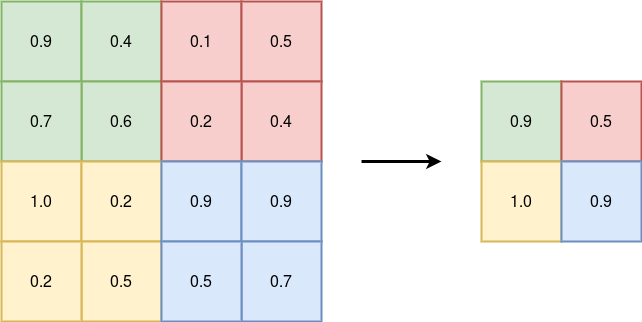
\includegraphics[scale=0.4]{figures/pooling.png}
    \caption{Example of a $2 x 2$ max pool operation with stride 2}
    \label{fig:maxpool}
\end{figure}

In figure \ref{fig:maxpool}, we see an input matrix $M$ where each 2x2 submatrix is being filtered by choosing the maximum element $\hat{M}_{max}$. The filter then strides across $M$ by two elements, repeating the operation until $M$ has been completely filtered.
\clearpage
\subsection{Autoencoder}

Autoencoders are specific types of neural networks used to learn efficient encodings of unlabeled data and then decode them to reconstruct the original data \cite{bank2021autoencoders}. Autoencoders consist of two models, the encoder $E_\phi$ and the decoder $D_\theta$. The relationship between these can be formulated as such: 

\begin{equation}\label{eq:enc}
E_\phi: X \rightarrow Z 
\end{equation}
\begin{equation}\label{eq:dec}
D_\theta: Z \rightarrow X
\end{equation}

$E_\phi$ compresses data $X$ into a latent representation $Z$. $D_\theta$ then decodes $Z$, thus outputting a reconstructed dataset of the same dimensions as the input. $E_\phi$ can be seen as a compressing model, while $D_\theta$ can be seen as a decompressing model. This is further showcased in figure \ref{fig:aediagram}. 

\begin{figure}[!h]
    \centering
    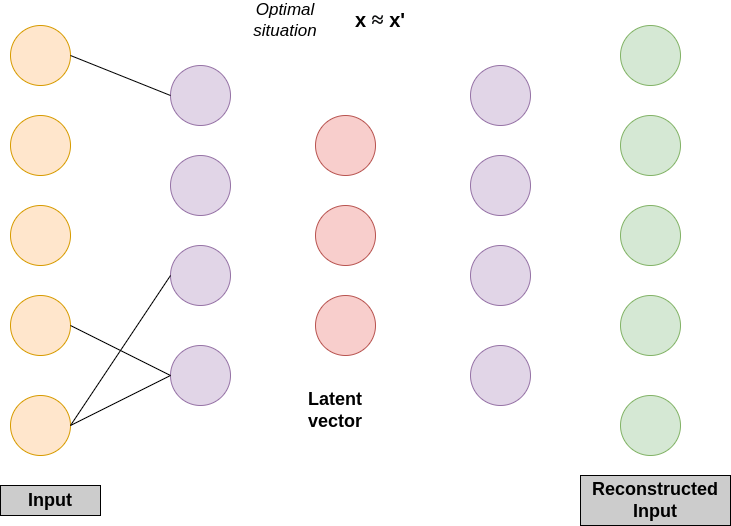
\includegraphics[scale=0.4]{figures/ae.png}
    \caption{Example of a dense autoencoder architecture}
    \label{fig:aediagram}
\end{figure}

The optima for any kind of autoencoder becomes that of lossless encoding, which can be described as such:

\begin{equation}
    X' = D_\theta(E_\phi(X))
\end{equation}

As mentioned in Section \ref{back:linear}, dense networks can struggle with feature extraction. This is also the case for dense autoencoders. By introducing convolutional layers, the autoencoder becomes more adept at image reconstruction and denoising \cite{zhang2018better}. These networks are called convolutional autoencoders (\acrshort{cae}).  \\

When the model is sufficiently trained for a specific task, $D$ \textit{may} become unnecessary for certain applications such as data reconstruction and denoising \cite{vincent2010stacked}. If the primary goal is feature extraction or dimensionality reduction, $E$ alone can be used to map input data to the lower-dimensional latent space. By utilizing only $E$, the overall complexity and size of the model $M$ can be reduced, which may be beneficial in scenarios with computational or memory constraints. For other tasks, such as autoencoders, include image reconstruction \cite{7797236}, signal analysis \cite{andrysiak2016machine}, and anomaly detection \cite{bank2021autoencoders}, the whole model is often needed.
\subsubsection{Latent Space}

The latent space $Z$ in autoencoders aims to capture essential features of the input data $X$ in a lower-dimensional representation. However, traditional autoencoders face limitations in their generative capabilities [CITE]. While they are trained to reconstruct original data accurately, they typically lack the ability to generate new, diverse samples from $Z$.
This limitation arises from the fact that regular autoencoders do not impose any specific structure on $Z$ beyond compressing the $X$. As a result, the latent representations may not be continuous or meaningful for interpolation and generation tasks.



\subsubsection{Loss functions for autoencoders}

The goal of an autoencoder is to make the reconstructed output $\hat{X}$ as close to the input $X$ as possible. Given this, the loss function used for these networks can be seen as a distance metric, where the objective is to minimize the distance $d$ between input and output:

\begin{equation}
    \mathcal{L}(\theta; X) = d(X, \hat{X}) = d(X, f_\theta(X))
\end{equation}
The optimization problem can then be formulated as:
\begin{equation}
    \theta^* = \argmin_{\theta} \mathbb{E}_{X \sim p_{\text{data}}(X)}[\mathcal{L}(\theta; X)]
\end{equation}
where $\theta^*$ are the optimal parameters for the network. Some of the more common loss functions used for autoencoders includes: \\

\clearpage


In addition to the issues with regular autoencoders in regards to decoding the latent space, these autoencoders have several disadvantages, including:

\begin{itemize}
    \item \textbf{Overfitting}: If the encoder and decoder become too powerful, they can learn to simply copy the input data to the output data.
    \item \textbf{Lack of regularization}: This can lead to poor generalization to unseen data
    \item \textbf{Input sensitivity}: Noise in the input data may potentially lead to large changes in the latent space
    \item \textbf{Interpretability}: The latent space may not be interpretable or correspond to meaningful features of the data
    \item \textbf{Encoding determinism}: Regular autoencoders don't account for uncertainty or multiple plausible interpretations of the input.
\end{itemize}
\clearpage
\subsection{Variational Autoencoder}
\label{back:vae}

The \acrfull{vae} \cite{kingma2022autoencodingvariationalbayes} is a type of autoencoder that aims to solve the lack of generative capabilities within regular autoencoders. \acrshort{vae}s are generative models that sample the latent space through a probabilistic distribution. This makes them suitable for image generation tasks \cite{vahdat2020nvae}, something regular autoencoders are unable to do due to their deterministic latent representation.

\begin{figure}[!h]
    \centering
    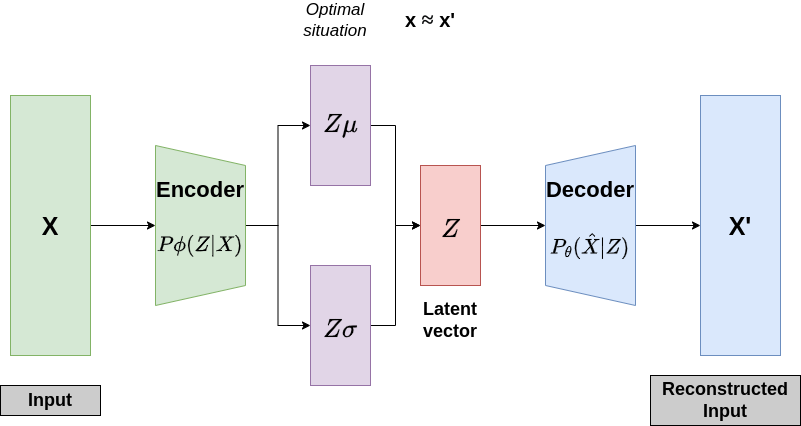
\includegraphics[scale=0.4]{figures/vae.png}
    \caption{Variational Autoencoder Architecture Diagram}
    \label{fig:vaediagram}
\end{figure}


\subsubsection{Reparametrization Trick}
\label{back:reparam}

\acrshort{vae}s can be trained efficiently using backpropagation due to a technique known as the \textit{reparameterization trick} \cite{kingma2022autoencodingvariationalbayes}. This is necessary because \acrshort{vae}s involve sampling from a stochastic latent variable $z$, which would normally hinder gradient-based optimization.

The idea is to express the sampling of $z$ from the approximate posterior $q_\phi(z|x) = \mathcal{N}(\mu, \sigma^2)$ as a deterministic function of the encoder outputs ($\mu$ and $\sigma$) and an additional noise variable $\epsilon$. Specifically:
\begin{equation}
    z = \mu + \sigma \odot \epsilon, \quad \epsilon \sim \mathcal{N}(0, I)
\end{equation}

Here, $\odot$ denotes element-wise multiplication. This formulation allows gradients to flow through the sampling process, enabling end-to-end training of the model.

The reparameterization trick transforms the optimization problem from one involving expectations over $q_\phi(z|x)$ to one involving expectations over $p(\epsilon)$, which is fixed and independent of the model parameters ($\phi$ and $\theta$):

\begin{equation}
    \mathbb{E}_{z \sim q_\phi(z|x)}[f(z)] = \mathbb{E}_{\epsilon \sim \mathcal{N}(0,I)}[f(\mu + \sigma \odot \epsilon)]
\end{equation}

This formulation makes training of \acrshort{vae} models feasable, even for gradient based optimizers, such as \acrshort{adam} or \acrshort{sgd}.




\subsubsection{Evidence Lower Bound}
\label{back:elbo}
In the context of \acrshort{vae}s, \acrshort{elbo} is commonly used as a loss function. \cite{lygerakis2024edvaeentropydecompositionelbo}. It consists of two parts, the reconstruction likelihood $\mathcal{L}_{\text{rec}}$ and the prior constraint $\mathcal{L}_{\text{reg}}$:
\begin{align}
\mathcal{L}_{\text{ELBO}}(\theta, \phi; x) &= \mathcal{L}_{\text{rec}}(\theta, \phi; x) + \mathcal{L}_{\text{reg}}(\phi; x)  
\end{align}
where:
\begin{align}
\mathcal{L}_{\text{rec}}(\theta, \phi; x) &= \mathbb{E}_{q_\phi(z|x)}[\log p_\theta(x|z)] \\
\mathcal{L}_{\text{reg}}(\phi; x) &= -D_{\text{KL}}(q_\phi(z|x) \| p(z))
\end{align}
$\mathcal{L}_{\text{reg}}$ is the negative \acrfull{kld} \cite{10.1214/aoms/1177729694}, which can be further formulated as:
\begin{equation}
    D_{\text{KL}}(q_\phi(z|x) \| p(z)) = \mathbb{E}_{q_\phi(z|x)}\left[\log \frac{q_\phi(z|x)}{p(z)}\right]
\end{equation}
$D_{\text{KL}}$ is always non-negative $(\geq 0)$ and is a statistical method used to quantify the proximity between two probability distributions \cite{shlens2014notes}. 
The reconstruction likelihood $\mathcal{L}_{\text{rec}}$ can be computed in different ways depending on the nature of the input data. For binary data, it is typically computed as a binary cross-entropy loss:
\begin{equation}
\mathcal{L_\text{rec}}(\theta, \phi; x) = - \mathbb{E}_{q_\phi(z|x)}[\mathcal{L}_{\text{BCE}}(x, z)]
\end{equation}
where $\mathcal{L}_{\text{BCE}}(x, z)$ is defined as:
\begin{equation}
\mathcal{L}_{\text{BCE}}(x, z) = \frac{1}{N} \sum_{i=1}^{N} \left( x_i \log p_\theta(x_i|z) + (1 - x_i) \log(1 - p_\theta(x_i|z)) \right)
\end{equation}
For continuous data, more novel adaptations \cite{lygerakis2024edvaeentropydecompositionelbo} often use the \acrshort{mse} loss as shown in equation \ref{eq:mse}, thus giving:
\begin{equation}
    \mathcal{L}_{\text{rec}}(\theta, \phi; x) = \mathbb{E}_{q_\phi(z|x)}[\|x - \hat{x}\|^2]
\end{equation}
where $\hat{x} = p_\theta(x|z)$ is the reconstructed input.
The two losses combined aims at providing a total loss that balances reconstruction quality and the prior regularization \cite{lin2019balancingreconstructionqualityregularisation}.

\subsubsection{Minimizing the ELBO Loss}
The objective in training a \acrshort{vae} is to minimize the negative \acrshort{elbo}, which is equivalent to maximizing the \acrshort{elbo} itself. This optimization problem can be formulated as:

\begin{equation}
    \theta^*, \phi^* = \argmin_{\theta, \phi} \mathbb{E}_{x \sim p_{\text{data}}(x)}[-\mathcal{L}_{\text{ELBO}}(\theta, \phi; x)]
\end{equation}

where $\theta^*$ and $\phi^*$ are the optimal parameters for the decoder and encoder, respectively. By minimizing the negative \acrshort{elbo}, we simultaneously optimize for better reconstruction of the input data (through $\mathcal{L}_{\text{rec}}$) and a latent space distribution that closely matches the prior (through $\mathcal{L}_{\text{reg}}$). This process encourages the \acrshort{vae} to learn a meaningful and structured latent representation of the input data while maintaining the ability to generate new samples \cite{kingma2022autoencodingvariationalbayes}.
\subsection{Data Processing and Mixed Precision Training}
\label{back:data}

\subsubsection{Data Normalization}

Normalization is a technique of which data is transformed from it's original scale, to a more standard scale \cite{ali2014data}. These techniques are normally used when the dataset has elements of different ranges. Normalization can contribute to faster convergence, and it's why they are as commonly used when preprocessing data. 

\textbf{MinMax Normalization} 

This algorithm transforms data to a specified range, most often $[0, 1]$ but it can also be $[-1, 1]$ or any other range.
Minmax normalization can be described as follows:

\begin{equation}
   x_{\text{normalized}} = \dfrac{x - x_{min}}{x_{max}-x_{min}}
\end{equation}
\vspace{0.2cm}

where $x$ denotes the data, $x_{min}$ and $x_{max}$ is the minimum and maximum in $x$. \\

\subsubsection{Half Precision Training}

Working with large datasets and \acrshort{dnn}s can be rather time- and resource consumptive. To address this, one can cast the datatype from single precision to half precision, along with weights, biases and losses. This will reduce loss of accuracy and information, but it can drastically lower memory consumption and decrease training time. It is important to note that casting of data occurs with normalization techniques, the order of which operation happens first is quintessential. If the data is casted to half precision before normalization, the normalization will be based on a slightly inaccurate representation of the data, but the computation of the normalized data will be faster. If normalization were to occur first, less detail about the data would be lost, but at the expense of being more computational intensive. \\

\textbf{Mixed precision training}

Mixed precision training, introduced in 2018 \cite{micikevicius2018mixed}, is a technique where the weights, activations and biases of a neural network is stored in single precision, while the data itself stays in it's original format. It allows for reduced memory consumption, while also speeding up operations of deep neural nets. Additionally, the amount of $\si{\kilo\watt\hour}$ required to train the neural nets would decrease, thus reducing both the cost and the environmental tax by training neural nets. This becomes more important the larger the datasets, models and the sheer amount of GPUS required to train massive workloads. This introduce the concept of loss scaling, where the losses needs to be adjusted based on the weights. \\

\mycomment{
\subsection{Dataloaders}

If the datasets contain information about the data and how to retrieve a single instance, the dataloaders job is to create an object that can be iterated over, containing $n$ amount of batches, and transferring these data to the wanted devices. In the case of data parallel multi-gpu training, when the data is loaded, it's \textit{sharded} across the different gpus, in a manner that balances the load of each gpu. Let's say we have a batch  of size $[4, 5, 5]$ and we have two gpus available. The dataloader can split this Tensor in two batches, where each of the gpus get a tensor of size $[2, 5, 5]$. By sharding the data along the first axis, ideally we can half the amount it takes, not taking data transfer time into consideration. 

\begin{figure}[!h]
    \centering
    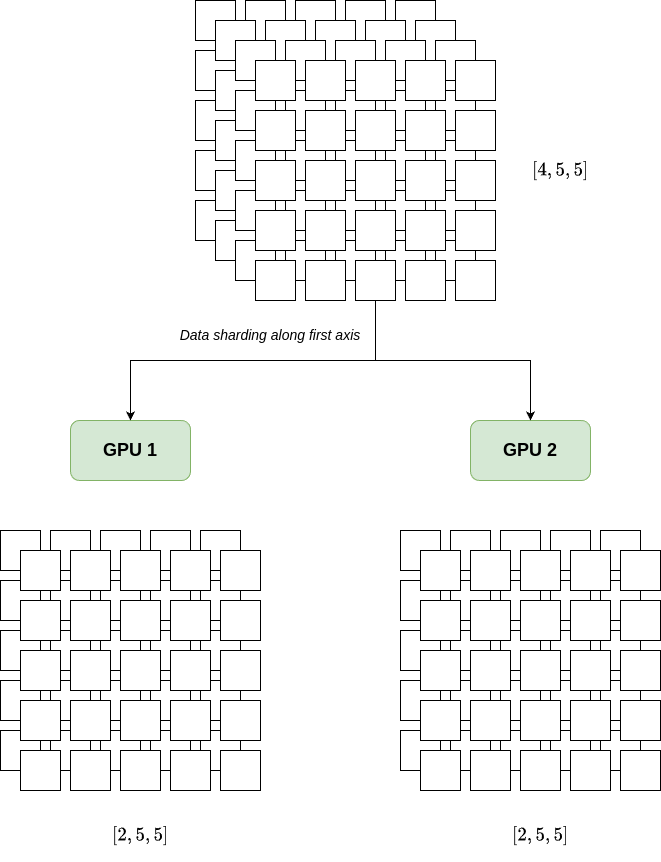
\includegraphics[scale=0.4]{figures/sharding.png}
    \caption{Example of data sharding with 2 gpus, and a original Tensor of size [4,5,5]}
    \label{fig:sharding}
\end{figure}


\textbf{Parallel loading}

When iterating over a dataloader, each element of the batch is retrieved and undergoes transformations. Depending on the batch size and  the size of the data, this procedure can be very resource-intensive and time-consuming. To mitigate this, we can introduce the concept of parallel batch loading. Instead of gathering and transforming the data sequentially, one can leverage available resources to do this operation in a parallel manner. Algorithm \ref{alg:parallel-batch-loading} details how such an operation is conducted.


\begin{algorithm}
\caption{Parallel Batch Data Loading}\label{alg:parallel-batch-loading}
\begin{algorithmic}
\Require BatchIndices, N
\Ensure BatchData, LoadSingleData
\State Initialize empty list BatchData
\State Create ThreadPool with N threads
\For{each Index in BatchIndices}
    \State Submit LoadSingleData(Index) to executor
\EndFor
\For{each completed Future from executor}
    \State Data $\gets$ Future.result()
    \State Append Data to BatchData
\EndFor
\State \Return BatchData
\end{algorithmic}
\end{algorithm}
}

\subsubsection{Overfitting and Early Stopping}

Overfitting is a common problem within \acrlong{ml} \cite{srivastava2014dropout}. It occurs when a model is trained , and fails to fit additional data. In addition to popular techniques such as dropout \cite{srivastava2014dropout}, \textit{early stopping} is a regularization technique that aims to avoid overfitting. When training an optimizer such as \acrshort{adam} \cite{kingma2017adam}, or \acrshort{sgd} \cite{Rumelhart1986, Bottou2012}, one can notice when a model is overfitting by studying the validation loss. If the validation loss $L_v$ starts increasing, the early stop mechanism will stop the training altogether if no improvement of $L_v$ is found after $p$ number of epochs. A formal definition can be given as such:

\begin{align*}
&\text{Stop at epoch } T \text{ if:} \\
&\forall i \in \{T-p+1, ..., T\}: L_v(i) > L_v^* - \epsilon \\
&\text{where } L_v^* = \min_{j=1}^{T} L_v(j) \\
\\
&\text{Given:} \\
&L_v(t) \text{ is the validation loss at epoch } t \\
&p \text{ is the patience (number of epochs to wait)} \\
&\epsilon \text{ is a small threshold for improvement}
\end{align*}

\subsubsection{Parallelism within \acrlong{ml}}

With rapid evolving deep learning architectures, the importance of scalable model training and networks grows larger each year. It is even estimated that these networks grow 1,5x each year \cite{9499913}, making parallelization a vital topic when it comes to \acrlong{ml} to accommodate ever increasing memory needs. Several different hardware accelerators have been created to best accommodate these needs, the most apparent of these are \acrshort{gpu}s. NVIDIA have for several years dominated this market, and their hardware is becoming faster and increasing in memory. \\

By workers, we mainly refer to \acrshort{gpu}s, but this could also be processors or other types of hardware accelerators such as TPUs.


\subsubsection{Model Parallelism}

\acrshort{dl} models need to store a lot of data. Weights and biases tend to take up a lot of memory, thus requiring the need of splitting up a model across several workers. As an example, given a model $M$ of 50 layers, we can split this model in 2 parts by having a worker $A$ manage the first 25 layers, and worker $B$ manage the latter half.
The overhead of transferring data across these workers can become a bottleneck, so this should only be utilized when absolutely necessary.

\subsubsection{Data Parallelism}

Data parallelism refers to partitioning data across multiple workers. Given a dataset $X$, we can split $X$ across the workers and store a copy of the model $M$ on each worker, calculate gradients across them all and update the trainable parameters for $M$. 

\subsubsection{Hybrid Parallelism}

This kind of parallelization combines the two previously mentioned techniques. First, $M$ is split across several workers, and then $X$ is subsequently split across multiple workers. 
\section{Anomaly Detection}
\label{back:anomdet}

\textit{Anomaly detection} is about identifying observations that can be deemed inconsistent with the rest of the dataset \cite{anomaly}. These anomalies can also be referred as outliers, surprises, exceptions, depending on domain. Anomaly detection can be used on all kinds of data, ranging from images to time-series data. There are 3 main types of anomalies, and those are \textit{point anomalies}, \textit{contextual anomalies} and \textit{collective anomalies}.

\begin{figure}[!h]
    \centering
    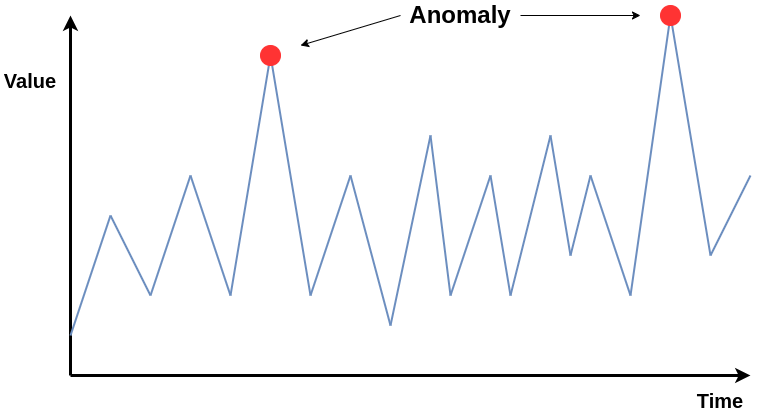
\includegraphics[scale=0.4]{figures/anolay_line.png}
    \caption{Example of anomalies in a time series}
    \label{fig:anomaly_example}
\end{figure}

While point anomalies target single instances that differ from the rest of the dataset, collective anomalies targets groups of instances that together form an anomaly. Contextual ones, as in the word, require context to determine whether or not an anomaly has been detected, and is typically found in time-series data.

Anomaly detection can be performed in a lot of different ways. From common machine learning tasks such as K-means clustering \cite{7507933}, \Gls{svm} \cite{10.1007/978-3-540-28647-9_97}





Given a matrix $a$ of data:

\[
A = \begin{bmatrix}
a_{11} & a_{12} & \cdots & a_{1n} \\
a_{21} & a_{22} & \cdots & a_{2n} \\
\vdots & \vdots & \ddots & \vdots \\
a_{m1} & a_{m2} & \cdots & a_{mn}
\end{bmatrix}
\]

We are interested in finding a region $a_{ij} to a_{kl}$ where $i < k \And j < l$ st. the values within these regions falls outside of the general range


For \acrshort{das} data specifically, anomaly detection can be used for detecting clusters of signals that don't correspond to the predisposed target feature. Registering these outlier signals and receiving real time information about these could prove vital in some cases,  and in best case scenario save lives. 

Dealing with sensitive data 

\subsection{Time series based anomaly detection}

Time series in one dimension is often a great candidate for anomaly detection. Stock market prediction, climate changes and several other series can be used to train networks to recognize point wise anomalies. Layers such as LSTM, RNN and GRU are constructed to store and retrieve information at a later time, thus introducing a memory mechanism. 

\subsection{Image based anomaly detection}

Anomaly detection can also be applied to images. Given a dataset of images with sheep, a image based anomaly detection model would be able to recognize any drastic changes between images. Without the temporal aspect of these problems, convolutional or linear layers are more often used. 

\begin{figure}[!h]
    \centering
    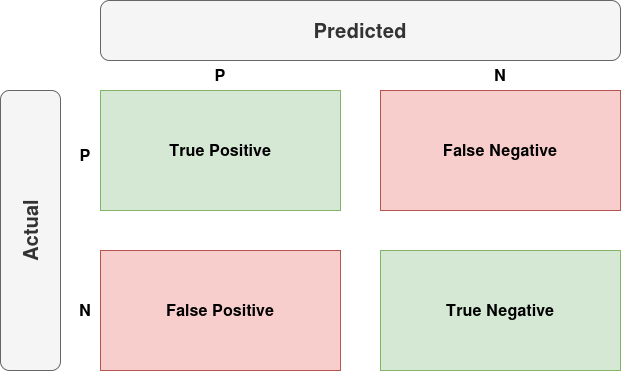
\includegraphics[width=0.5\linewidth]{figures/confmat.png}
    \caption{Caption}
    \label{fig:confmat}
\end{figure}

\section{Related Work}
\label{relwork:anomaly}


\subsection{\acrshort{das} file loading and processing}

One of the file formats used for storing \acrshort{das} data is \acrshort{hdf5}. Many of the implemented libraries for \acrshort{hdf5} files now allow for parallel loading of these files. Biddiscombe (et. al 2012) replaced the IO layer within a \acrshort{hdf5} library ''to allow for parallel loading between simulation and analysis'' \cite{biddiscombe2012parallel}. In later years, \texttt{HDF5.jl}, the HDF5 library in Julia, allows for parallel loading of files, utilizing the message-passing interface (MPI). This can potentially reduce \acrshort{das} file loading times. \\ 

An important aspect of \acrshort{das} processing revolves around frequency analysis, denoising, and other types of filtering. 2D \acrfull{fft}s within 2D linear band pass filtering, and one-dimensional adaptive filtering using \acrfull{fir} filters have all been studied and \cite{daspreproc}. In our preliminary studies, we conducted a performance comparison between Julia and Python for computing 2D Fast Fourier Transforms (FFTs) on \acrshort{das} data using \acrshort{gpu}s. Our results demonstrated that Julia significantly outperformed Python in this specific operation \cite{projthesis}. \\

Public \acrshort{das} datasets are often scarce and hard to find. PubDAS \cite{spica2023pubdas} is a public distribution of several \acrshort{das} datasets worldwide, stored in multiple file formats. Many of these datasets contain scripts containing preprocessing algorithms or visualization code. These techniques are sequential, preprocessing file by file and possibly removing erroneous files. These scripts are mainly single-file Python or MatLab scripts. \\ 

One key aspect of \acrshort{ann}s is the necessity of larger train datasets. Data augmentation techniques such as cropping, resizing, or color grading can increase the available datasets for more vision-based tasks. Another way to increase the total amount of train data is by leveraging \acrshort{gan}s. After training a \acrshort{gan} model, the generator can produce data similar to already collected data. This has yielded great results on \acrshort{das} data \cite{Shiloh:19}, and can be a great way to provide more train data, which in turn can help models detect anomalies more accurately by being trained on a wider variety of data. \\

\subsection{Anomaly detection algorithms for \acrshort{das} data analysis}

The most commonly used algorithms regarding machine learning have traditionally been centered around Kmeans clustering, K nearest neighbors, and  Support Vector machines \cite{10.14778/3538598.3538602, 10.1145/3444690}. These have proven to be efficient, especially when dealing with unlabeled data. These clustering techniques are good at outlining groups grouping them, and finding outliers while dealing with them. One article found k means to be a great choice when dealing with traffic analysis and detection \cite{7507933}. Others have looked at svms as another solid option when dealing with anomaly detection \cite{10.1007/978-3-540-28647-9_97}. Omar (et al 2013) \cite{omar2013machine} looked in general at machine learning techniques such as SVMs, k means, decision trees and bayesian networks, and found that supervised ones generally outperforms their unsupervised counterparts when the types of anomalies where known beforehand, but struggle with novel anomalies. \\ 

Alongside well-known clustering techniques such as k means and knn, \acrfull{dbscan}, first published in 1996 \cite{10.5555/3001460.3001507} is a well-known clustering technique suited for outlier detection in multidimensional datasets. It's still being researched and improved as of this date for multivariate time series \cite{waltz2024time}, and has numerous implementations in different frameworks and languages.  


%%%%%%%%%%%%%%%%%%%%%%%%%%%%
%% AE DAS $$$$$ 
%%%%%%%%%%%%%%%%%%%%%%%%%%%%%%%%%%%%%%%%%%%%
An effort has been made into trying to improve autoencoders for anomaly detection \cite{tan2023improving}

Vae for time series \cite{desai2021timevae}


Ball2017 - dl in remote sensing

apSensingo2019railwaydas - powerpoint
s21196627 - dnn microseismic , das
sensors - mdpi ???

In general, autoencoders with linear, convolutional, or recurrent layers, clustering algorithms, and more traditional \acrshort{ml} methods have seen many use-cases within \acrshort{das} research. However, in later years with the later additions of both attention layers, or even \acrshort{gan}s \cite{goodfellow2014generative, goodfellow2016nips}, more novel approaches are being researched. By introducing channel attention and spatial attention to \acrshort{cnn}, one article \cite{eage:/content/journals/10.1111/1365-2478.13355} finds good results for denoising \acrshort{das} signals. 


Label-free autoencoder-based anomaly detection on \acrshort{das} data has been conducted as late as in 2023 \cite{xie2023label}. A combination of a convolutional autoencoder trained on normal-range \acrshort{das} data and a clustering algorithm to locate the feature center was found to beat state-of-the-art supervised networks. Another interesting aspect of this research is the emphasis on model size, creating a sufficient \acrshort{cae} model with only \qty{1.34}{\si{\kilo}} parameters. This research, in particular, has led the ground for our research and the creation of a program for training and comparing several types of autoencoders. \\





\subsection{Other Models}

Zhu (et al. 2023) use ''a pre-trained PhaseNet to generate noisy labels of P/S arrivals in \acrshort{das} data'' and ''applied the GaMMa method to refine noisy labels and build training datasets'' \cite{zhu2023seismic}. A \acrshort{dl} model was then made to detect earthquakes. \\


\acrshort{gan} is another type of generative nn, first proposed by Iain Goodfellow around 2016 \cite{goodfellow2016nips}. These networks have been utilized in models for specifically designed for anomaly detection. A \acrshort{lstm} \acrshort{vae} \acrshort{gan} model was built to detect anomalies within time series \cite{s20133738}. A modification of \acrshort{lstm} \acrshort{gan}, with the inclusion of the attention mechanism \cite{vaswani2017attention}, was built for time-series anomaly detection \cite{bashar2023algan}.ALGAN-DA?
AEGAN-AD \cite{jiang2023unsupervised} uses a \acrshort{gan} based approach to detect anomalies within audio.

Researchers at NTNU constructed a \acrshort{lstm} \acrshort{vae} model for fault detection on a multi-sensor system for maritime systems \cite{9514856} with good success. Deep \acrshort{lstm}-based autoencoders have also been found to be able to detect anomalies within multivariate time-series forecasting problems \cite{alaaDeepLstm2019}.

One issue of concern is online long-distance distributed monitoring applications. By using a combination of a ResNET with a convolutional block attention module (CBAM), one paper is able to achieve real-time inference time cost as low as 3.3ms per sample \cite{photonics9100677}, while still averaging a high accuracy, even for multi-scenario scenes. 


% Huang (et al. 2021) \cite{huang2021esad} semisupervised learning  kl


Anomaly detection, sometimes referred to as outlier detection, is highly relevant within \acrshort{das} research. In 2017, several classical \acrshort{ml} techniques such as Gaussian Mixture Model (GMM), Hidden Markov Model (HMM), Naive Bayes (NB), and Restricted Boltzmann Machine (RBM) were compared to discriminative models, including \acrshort{ann}s \cite{app7080841}. Variations of isolation forests are shown to be able to perform fault detection for mining conveyors\cite{WIJAYA2022110330}. \\

As previously mentioned in chapter \ref{chap:introduction}, label-free anomaly detection has the advantage of requiring a lot less manual labor and can be adapted to multiple datasets. A model that requires only normal-state data, utilizing both autoencoders and the K-means clustering technique, has yielded great results, even beating supervised methods \cite{s23084094}. \\ 

a, \cite{10.14778/3538598.3538602} \cite{10.1145/3444690}.

All this research shows how processing and anomaly detection on \acrshort{das} data is highly relevant. However, most of them do not necessarily concern themselves with available computational power, overall memory consumption, or how to optimize these algorithms for real-time environments, where accuracy, fault tolerance, and inference speed are of utmost importance.



THIS ONE IS HIGHLY RELEVANT AND HAS MANY METRICS \cite{s23021009}
